\section*{Łączenie wyjaśnień różnych metod}

W celu uzyskania bardziej kompleksowego zrozumienia i interpretacji modeli głębokiego uczenia, zastosowano podejście polegające na łączeniu wyjaśnień generowanych przez różne metody XAI: GradCAM, LIME i SHAP.
Łączenie wyjaśnień pozwala na wydobycie wspólnych elementóœ interpreatacji, które mogą dostarczyć bardziej wiarygodnych informacji o decyzjach modelu.

W badaniach przeanalizowano dwa podejścia do łączenia wyjaśnień:
\begin{enumerate}
	\item Część wspólna - polega na wyznaczeniu wspólnych obszarów wyjaśnień generowanych przez różne metody.
	      Obszary te mogą być uznane za  bradziej pewne, ponieważ zostały wskazane przez więcej niż jedną metodę.
	\item Suma obszarów - polega na połączeniu wszystkich obszarów wyjaśnień generowanych przez różne metody.
	      Dzięki temu podejściu można uzyskać bardziej rozległe wyjaśnienia, które łączą informacje z różnych metod.
\end{enumerate}

Przeprowadzono analizę tych podejść, aby ocenić, w jaki spośob różne metody mogą być łączone, aby dostarczyć lepszych wyjaśnień decyzji modeli głębokiego uczenia.

\subsection*{Część wspólna}
Analiza częsci wspólnej wyjaśnień koncentruje się na identyfikacji obszarów na obrazach, które są wspólne dla metod XAI takich jak GradCAM, LIME i SHAP.
Ta metoda pozwala na odkrycie kluczowych elementów decyzyjnych modeli, które są potwierdzone przez różne techniki wyjaśniania.

\begin{figure}[h]
	\centering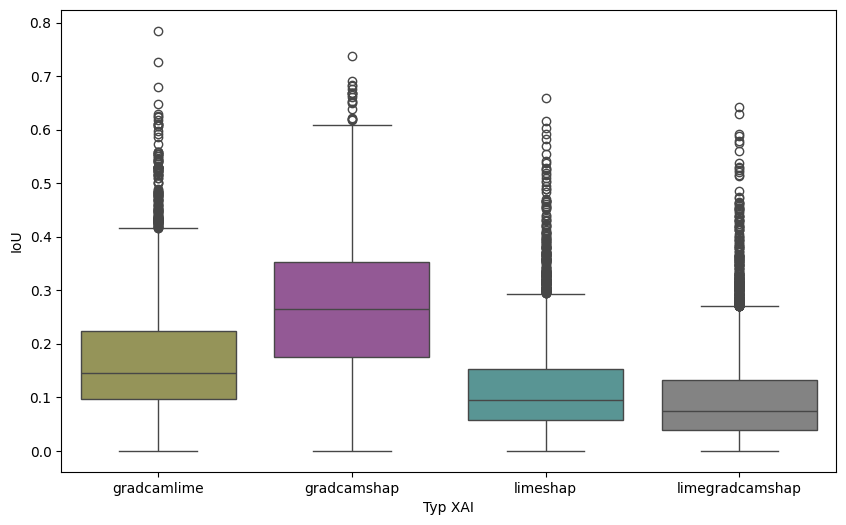
\includegraphics[width=.9\textwidth]{img/combine_iou_and}
	\caption{IoU dla połączeń wyjaśnień poprzez część wspólną}  \label{rys:combine_iou_and}
\end{figure}
\begin{table}[h]
	\centering
	\begin{tabular}{|c|c|}
		\hline
		\textbf{Metoda XAI}  & Średnie IoU \\
		\hline
		GradCAM i LIME       & 0.150297    \\
		\hline
		GradCAM i SHAP       & 0.091504    \\
		\hline
		LIME i SHAP          & 0.035271    \\
		\hline
		GradCAM, LIME i SHAP & 0.029152    \\
		\hline
	\end{tabular}
	\caption{Średnie wartości IoU części wspólnej połączonych wyjaśnień}
	\label{tab:combineandiouand}
\end{table}
Tabela \ref{tab:combineandiouand} średnie wartości dla połączonych wyjaśnień różnych metod XAI.

Najlepsze wyniki osiągnąło połączenie wyjaśnień GradCAM oraz LIME.
Najgorsze wyniki osiągneło połączenie wszystkich trzechwyjaśnień.
Żadne z połączeń nie uzyskało lepszego średniego wyniku  IoU niż średni wynik którgokolwiek z części wyjaśnień.
Powodem jest zbyt duże zmniejszenie wielkość wyjaśnień.

\vspace{1cm}

\begin{figure}[h]
	\centering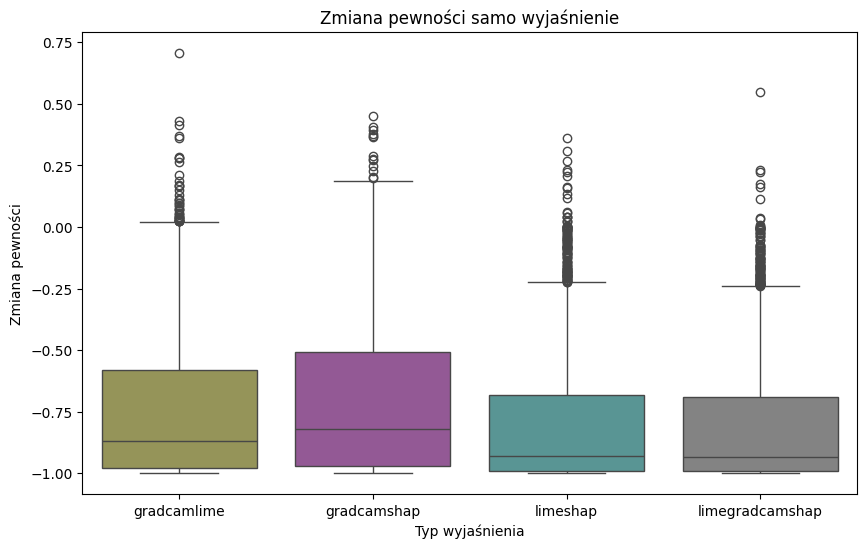
\includegraphics[width=.9\textwidth]{img/combine_confidence_exp_and}
	\caption{Zmiana pewności po pozostawieniu samego wyjaśnienia}  \label{rys:combineandconfidencean}
\end{figure}
\begin{table}[h]
	\centering
	\begin{tabular}{|c|c|}
		\hline
		\textbf{Metoda XAI}  & Zmiana pewności \\
		\hline
		GradCAM i LIME       & -0.789047       \\
		\hline
		GradCAM i SHAP       & -0.932662       \\
		\hline
		LIME i SHAP          & -0.840479       \\
		\hline
		GradCAM, LIME i SHAP & -0.789047       \\
		\hline
	\end{tabular}
	\caption{Zmień na procent}
	\label{tab:combineandconfidenceand}
\end{table}
Zmiana pewności po pozostawieniu samego wyjaśnienia została przedstawiona na \ref{rys:combineandconfidencean} oraz w tabeli \ref{tab:combineandconfidenceand}.
Najlepsze wyniki dla połączenia GradCAM z SHAP, jednak zadal gorsze niż wyjaśnienie uzyskane z samego GradCAM lub samgeo SHAPA.
Żadne z połączeń nie uzyskało lepszego średniego zmiany pewności niż średni wynik którgokolwiek z części wyjaśnień.

\vspace{1cm}

\begin{figure}[h]
	\centering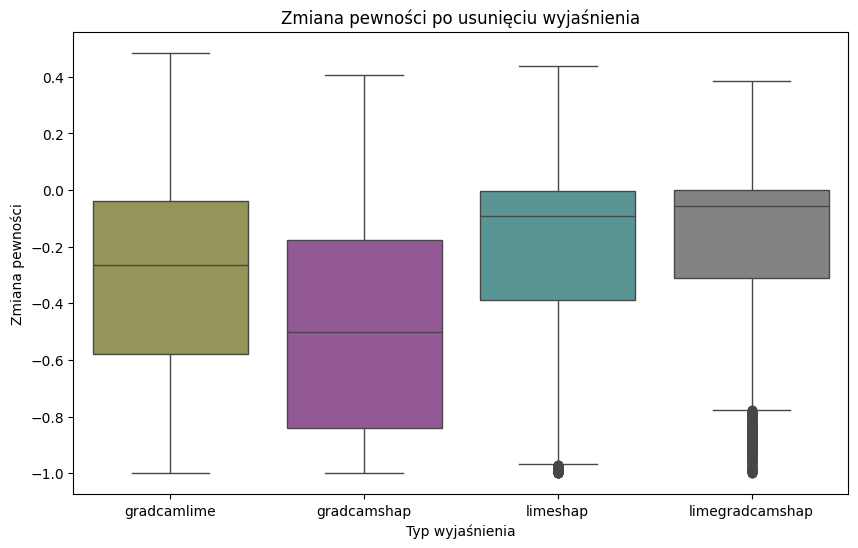
\includegraphics[width=.9\textwidth]{img/combine_confidence_no_exp_and}
	\caption{Zmiana pewności przy usunięciu obszarów wyjaśnienia}  \label{rys:combineandconfidenceandno}
\end{figure}
\begin{table}
	\centering
	\begin{tabular}{|c|c|}
		\hline
		\textbf{Metoda XAI}  & Zmiana pewności \\
		\hline
		GradCAM i LIME       & -0.290897       \\
		\hline
		GradCAM i SHAP       & -0.153363       \\
		\hline
		LIME i SHAP          & -0.068956       \\
		\hline
		GradCAM, LIME i SHAP & -0.059519       \\
		\hline
	\end{tabular}
	\caption{Średnia zmiana pewności usunięciu części wspólne wyjaśnień}
	\label{tab:combineandconfidenceandno}
\end{table}
Zmiana pewności przy usunięciu obszarów wyjaśnienia zostały przedstawiona na rysunku \ref{rys:combineandconfidenceandno} oraz w tabeli \ref{tab:combineandconfidenceandno}
Najlepsze wyniki były dla połączenia GradCAM oraz LIME, jednak nadal gorsze niż którekolwiek z części wyjaśnień.
Żadne z połączeń nie uzyskało lepszego średniego zmiany pewności niż średni wynik którgokolwiek z części wyjaśnień.

\vspace{1cm}
Podsumowując wyjaśnienia stworzone poprzez połączenie wyjaśnień częścią wspólną, dały gorsze wyniki niż same wyjaśnienia.
Wyjaśnienia wygenerowane w ten sposób skupiają się zbytnio na małych cechach, a nie całych obiektach aby były dobrze mierzalne w tej pracy.

\subsection*{Suma obszarów}
W tej sekcji przeanalizowano, jak różne metody XAI mogą zostać połączone poprzez sumę obszarów wyjaśnień.

\begin{figure}[h]
	\centering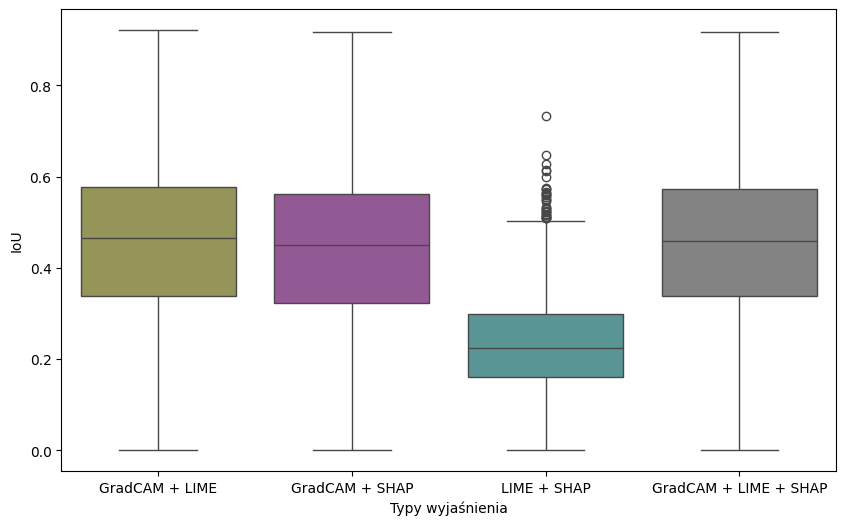
\includegraphics[width=.9\textwidth]{img/combine_iou_or}
	\caption{IoU dla połączeń wyjaśnień poprzez sume obszarów}  \label{rys:combine_iou_or}
\end{figure}
\begin{table}[h]
	\centering
	\begin{tabular}{|c|c|}
		\hline
		\textbf{Metoda XAI}  & Średnie IoU \\
		\hline
		GradCAM i LIME       & 0.452811    \\
		\hline
		GradCAM i SHAP       & 0.438179    \\
		\hline
		SHAP i LIME          & 0.233566    \\
		\hline
		GradCAM, LIME i SHAP & 0.448209    \\
		\hline
	\end{tabular}
	\caption{Średnie wartości IoU części wspólnej połączonych wyjaśnień}
	\label{tab:combineandiou}
\end{table}
Tabela \ref{tab:combineandiou} średnie wartości dla połączonych wyjaśnień różnych metod XAI.
Najlepszy wynik uzsykano z połączenia wyjaśnień GradCAM oraz LIME, które uzyskało wynik lepszy niż, sam GradCAM lub sam LIME.
Wszystkie połączenia dały lepsze wyniki niż dowolne jedno sani wyjaśnienie.

\vspace{1cm}

\begin{figure}[h]
	\centering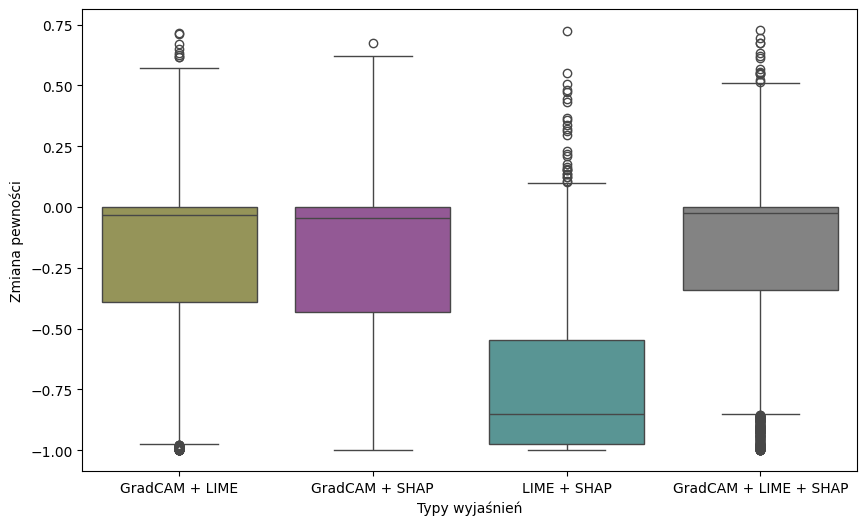
\includegraphics[width=.9\textwidth]{img/combine_confidence_exp_or}
	\caption{Zmiana pewności po pozostawieniu samego wyjaśnienia}  \label{rys:combineandconfidenceor}
\end{figure}
\begin{table}[h]
	\centering
	\begin{tabular}{|c|c|}
		\hline
		\textbf{Metoda XAI}  & Zmiana pewności \\
		\hline
		GradCAM i LIME       & -0.186505       \\
		\hline
		GradCAM i SHAP       & -0.210394       \\
		\hline
		SHAP i LIME          & -0.730767       \\
		\hline
		GradCAM, LIME i SHAP & -0.169937       \\
		\hline
	\end{tabular}
	\caption{Zmień}
	\label{tab:combineandconfidenceor}
\end{table}
Zmiana pewności po pozostawieniu samego wyjaśnienia została przedstawiona na \ref{rys:combineandconfidenceor}oraz w tabeli \ref{tab:combineandconfidenceor}.
Najlepszy wynik uzyskało połączenie wszystkich trzech wyjaśnień, co dało znacznie lepsze wyniki niż użycie jedngo wyjaśnienia.
Spowodowane to było mniejszą modeyfikacją.
Najgorsze wyniki uzyskało połączenie SHAP oraz LIME, nadal będąc lepszym wynikiem niż którekolwiek z pojedyńczych części.
\vspace{1cm}

\begin{figure}[h]
	\centering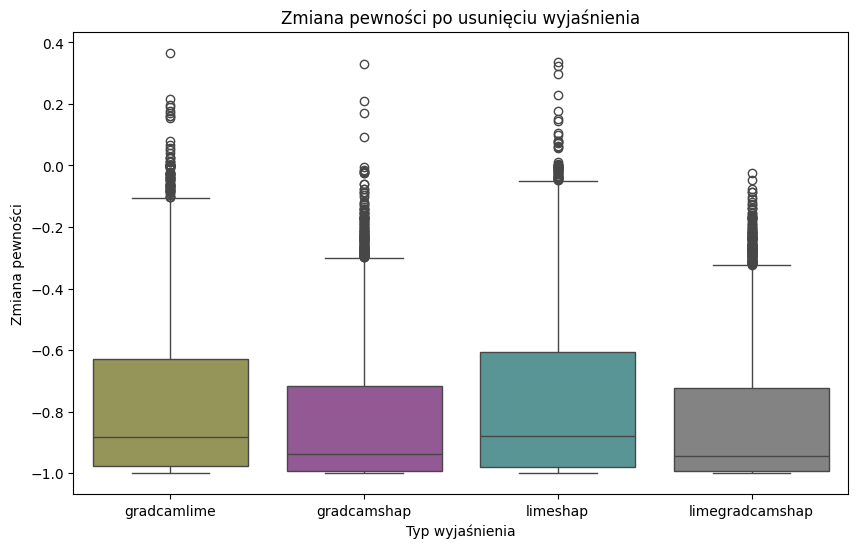
\includegraphics[width=.9\textwidth]{img/combine_confidence_no_exp_or}
	\caption{Zmiana pewności przy usunięciu obszarów wyjaśnienia}  \label{rys:combineandconfidenceorno}
\end{figure}
\begin{table}[h]
	\centering
	\begin{tabular}{|c|c|}
		\hline
		\textbf{Metoda XAI}  & Zmiana pewności \\
		\hline
		GradCAM i LIME       & -0.772289       \\
		\hline
		GradCAM i SHAP       & -0.780159       \\
		\hline
		SHAP i LIME          & -0.490221       \\
		\hline
		GradCAM, LIME i SHAP & -0.799201       \\
		\hline
	\end{tabular}
	\caption{Średnia zmiana pewności usunięciu obszarów}
	\label{tab:combineandconfidenceorno}
\end{table}
Zmiana pewności po pozostawieniu samego wyjaśnienia została przedstawiona na \ref{rys:combineandconfidenceorno}oraz w tabeli \ref{tab:combineandconfidenceorno}.
Najlepszy wynik uzyskało połączenie wszystkich trzech metod.
Dodatkowo tak jak wcześniej połączenie zawsze jest lepsze niż, który kolwiek element indywidualnie.

\vspace{1cm}
Podsumowując jest w tych badaniach wykazano że połączenie wyjaśnień poprzez sumę pozwala na znalezienie lepszych wyników.
Kosztem takiego połączenia jest wielkość wyjaśnienia, nie jest on tak precyzyjne i uogólnia.
